\documentclass[11pt,a4paper]{article}
\usepackage[margin=2.3cm]{geometry}
\usepackage[T1]{fontenc}
\usepackage{lmodern}
\usepackage{amsmath,amssymb,amsthm}
\usepackage{booktabs,tabularx,multirow}
\usepackage{graphicx}
\usepackage{xcolor}
\usepackage[hidelinks]{hyperref}
\usepackage[numbers,sort&compress]{natbib}
\usepackage{enumitem}
\usepackage[section]{placeins}  % keep each section's floats in that section
\setlist{nosep,leftmargin=*}
\newtheorem{proposition}{Proposition}
\newcommand{\pend}[1]{\textcolor{gray}{[pending: #1]}}

% ---- fill in -------------------------------------------------------------------------
\newcommand{\AUTHOR}{Saksham Bansal}
\newcommand{\IDNO}{f20220524@pilani.bits-pilani.ac.in}
\newcommand{\SUPERVISOR}{Prof.\ Hari Babu}
% ---------------------------------------------------------------------------------------

\title{Query-Adaptive Compression-Level Routing for Edge LLM Inference:\\
\Large When Does It Pay Off?\\[4pt]
\large B.Tech Thesis --- Mid-Semester Report}
\author{\AUTHOR\\ \small\texttt{\IDNO}\\[2pt] \normalsize Supervisor: \SUPERVISOR\\ BITS Pilani}
\date{\today}

\begin{document}
\maketitle

\begin{abstract}
Choosing an LLM's compression level per query promises cheaper edge inference, but it assumes that compressed variants remain useful and that the hardware turns fewer parameters into lower cost. We test both assumptions. We port FLAP, a retraining-free structured pruning method, to SmolLM2-1.7B and obtain a ladder of nested pruned variants of one model, stored as small pruning plans over a single copy of the weights. We build a 19{,}242-question pool from eight benchmarks with reproducible splits and a scoring pipeline that checks every result against the evaluation harness. On a Tesla T4, FLAP raises WikiText-2 perplexity from 18.48 to 25.94 at 20\% and 124.62 at 50\% of prunable parameters removed (Wanda-SP: 549.25 at 50\%; Magnitude-SP fails), reproducing the FLAP paper's method ranking at this scale. Pruning 50\% cuts 1024-token prefill latency by 38\% and energy per generated token by 27\%, but batch-1 decode latency stays at 30.4--31.1\,ms per token for every ratio. On 3{,}849 test questions, macro accuracy falls from 62.5\% (unpruned) to 47.3\% (FLAP 20\%), 40.0\% (FLAP 35\%), 32.6\% (FLAP 50\%); several pruned variants collapse to a constant answer on MMLU and BoolQ and fail to finish GSM8K answers. A per-query oracle over the variants reaches 75.8\% versus 64.1\% for the best fixed variant, but once variants that do not beat a constant answer are excluded the gain shrinks to 1.9 points (66.1\%) for this 20/35/50\% ladder. Calibrating FLAP on train-split questions instead of Wikipedia, with no retraining, raises macro accuracy by 2.4, 5.2, 4.3 points at 10/20/35\% (all McNemar $p\le$7.3e-08) and largely removes the constant-answer collapse at 10--20\%. With a ladder of the unpruned model and in-domain-calibrated FLAP at 10/20/35\%, the informative oracle reaches 71.9\% at 239\,ms per question against 64.1\% at 292\,ms for the unpruned model, an upper bound for a realistic router. Per-query compression-level routing therefore depends on in-domain calibration of the cheap tier and on a device that turns compression into cost savings. Laptop-CPU latencies are pending. 

\end{abstract}

\tableofcontents
\newpage

%=======================================================================================
\section{Introduction}
Small open language models (1--3\,B parameters) can now run on edge-class hardware, but every
query is still answered with the same, fixed amount of computation. Structured pruning methods
such as FLAP~\citep{an2024flap} and SliceGPT~\citep{ashkboos2024slicegpt} reduce that computation
without retraining, but they fix one compression ratio at deployment time. Queries, however, differ
in difficulty: a heavily pruned model may answer an easy question correctly and fail a hard one.

Choosing the compression level \emph{per query} is attractive, but it rests on two assumptions that are
usually taken for granted: that a heavily compressed variant of the model is still \emph{useful} on the
queries routed to it, and that the hardware turns the smaller model into a real \emph{cost} saving. This
thesis tests both assumptions on edge hardware. We build a ladder of FLAP-pruned variants of one model
(SmolLM2-1.7B~\citep{allal2025smollm2}), measure every variant on every query of a 19{,}242-question pool
drawn from eight standard benchmarks, and ask under which conditions a router can gain accuracy per cost
over simply running one fixed variant.

\paragraph{Core claim.} Per-query compression-level routing only pays off when (i)~the compression method
produces a cheap tier that still carries information --- for training-free FLAP on a 1.7\,B model this
means milder ratios (10--20\%) and in-domain calibration data --- and (ii)~the device turns fewer parameters
into lower cost, which on a
GPU at batch size~1 holds for prefill and energy but not for decoding. We measure the routing headroom with
an oracle corrected for constant-answer artefacts; whether a realistic router captures it is the subject of
the second half of the thesis.

In the resource-management taxonomy of Walia et al.~\citep{walia2024survey}, the compression level is
the resource being allocated and the router is a per-request scheduling/provisioning decision; that
survey and the MCDS scheduler~\citep{tuli2022mcds} do not treat LLM-inference workloads.

\paragraph{Status at mid-semester.} Phase 0 (infrastructure) is complete and verified. Phase 1 (FLAP port,
ratio sweep, baselines) and Phase 2 on the test split (query pool, scoring pipeline, external labels, outcome
runs of four variants, headroom analysis) are implemented, tested and run on a Colab T4. Laptop-CPU latency
and the train/validation outcome runs are deferred. Section~\ref{sec:results} reports only numbers that
exist in result files; everything else is marked as pending.

\paragraph{Research questions.}
\begin{enumerate}
  \item[RQ1] Can a training-free pruning method give a \emph{useful} ladder of compression levels for a
  $\sim$1.7\,B edge model, and what does it need (method, calibration data)?
  \item[RQ2] How much can a per-query choice of the compression level gain over the best fixed level once
  artefacts such as constant-answer variants are removed (informative-oracle headroom)?
  \item[RQ3] How much of that headroom does a realistic router recover, and does it beat routing on task type alone?
  \item[RQ4] On which devices does compression turn into lower latency, energy and memory, and therefore
  when can routing or cascading save cost?
\end{enumerate}
This report answers RQ1, answers RQ2 on the GPU and gives a first answer to RQ4 on the GPU; RQ3 and the
CPU part of RQ4 are planned (Section~\ref{sec:plan}).

%=======================================================================================
\section{Related Work}
\label{sec:related}
\paragraph{Resource management at the edge.} Walia et al.~\citep{walia2024survey} survey AI-based
resource management (provisioning, offloading, scheduling, placement, load balancing) in fog/edge
systems; Tuli et al.~\citep{tuli2022mcds} schedule workflow DAGs with Monte-Carlo tree search and a
learned surrogate. Neither addresses LLM inference.

\paragraph{Retraining-free structured pruning.} FLAP~\citep{an2024flap} scores channels by the
fluctuation of their inputs, chooses per-layer ratios through a global standardised threshold and adds
a bias that compensates for the removed channels. SliceGPT~\citep{ashkboos2024slicegpt} rotates and
deletes rows/columns. Wanda~\citep{sun2024wanda} (and its structured variant Wanda-SP, evaluated in
FLAP) uses weight$\times$activation importance; LLM-Pruner~\citep{ma2023llmpruner} needs LoRA recovery.
The choice of calibration data matters: Williams and Aletras~\citep{williams2024calibration} show that
pruning is more sensitive to it than quantisation, and Bandari et al.~\citep{bandari2024c4} find that the
common default (C4) is not always the best choice for LLM pruning.

\paragraph{Input-adaptive and elastic compression.} PuDDing~\citep{wee2025pudding} trains a router that
selects one of several \emph{depth}-pruned variants per prompt at a fixed sparsity.
Instruction-Following Pruning~\citep{hou2025ifpruning} predicts per-prompt structured masks with a
trained predictor. Flextron~\citep{cai2024flextron} and MatFormer~\citep{devvrit2024matformer} train
nested elastic models. RAP~\citep{liu2025rap} uses reinforcement learning to choose a pruning policy
from sequence length, batch size and the available memory budget.

\paragraph{Query routing.} RouterBench~\citep{hu2024routerbench} benchmarks routing across 11 LLMs and
evaluates routers against the convex hull of fixed models; RouteLLM~\citep{ong2024routellm} and Hybrid
LLM~\citep{ding2024hybridllm} route between a strong and a weak model; ConsRoute~\citep{qiao2026consroute}
and HybridFlow~\citep{dong2026hybridflow} route across device/edge/cloud model tiers.

%=======================================================================================
\section{Novelty and Positioning}
Per-prompt selection among pruned variants is \emph{not} new: PuDDing~\citep{wee2025pudding} does it
for depth pruning. Nor is the observation that calibration data affects pruning
\citep{williams2024calibration,bandari2024c4}. The contributions of this thesis are narrower:
\begin{enumerate}
  \item \textbf{A usable training-free ladder for a small edge model.} We show that FLAP on a 1.7\,B model,
  calibrated on Wikipedia as in the original method, collapses to constant answers on several tasks, and that
  calibrating it on in-domain questions (train split, no answers) largely removes this collapse at 10--20\%.
  The variants are \textbf{nested} (Proposition~\ref{prop:nested}), so one copy of the weights can serve all of them.
  \item \textbf{An artefact-corrected measurement of routing headroom.} An \emph{informative oracle} that only
  admits variants beating a constant answer, together with comparisons of ladders at matched ratios, separates
  real headroom from constant-answer artefacts that make a naive oracle overstate it.
  \item \textbf{An edge cost characterisation of compression-level routing.} On a GPU at batch size~1, width
  pruning lowers prefill latency, energy and memory but not decode latency; a query-level cascade saves cost only
  if the cheap tier serves more questions than its cost ratio, which we derive and measure. Choosing \emph{how
  much} to compress per query (variable budget, cost-aware) differs from choosing \emph{which} structure to keep
  at a fixed budget (PuDDing, IFPruning) or reacting to memory pressure (RAP).
\end{enumerate}
Prior routing work (RouterBench, RouteLLM, Hybrid LLM, ConsRoute, HybridFlow) routes between
\emph{separate} models; pruned variants of one model tend to fail on the same queries, so the headroom
available to a router is an empirical question (RQ2) rather than an assumption.

%=======================================================================================
\section{Problem Formulation}
\label{sec:problem}
Let $\mathcal{V}=\{v_0,\dots,v_K\}$ be pruned variants of one model, $v_0$ unpruned, ordered by cost.
For a query set $Q$:
\begin{itemize}
  \item $Y_{q,v}\in\{0,1\}$: whether $v$ answers $q$ correctly (task-specific primary metric, Sec.~\ref{sec:data});
  \item $c(q,v)$: the cost (latency in ms, or energy in J) of answering $q$ with $v$ on a given device.
\end{itemize}
A router is a map $\pi:Q\to\mathcal{V}$ with accuracy and cost
\begin{equation}
  A(\pi)=\frac1{|Q|}\sum_{q}Y_{q,\pi(q)},\qquad C(\pi)=\frac1{|Q|}\sum_q c\big(q,\pi(q)\big)+c_{\text{router}} .
\end{equation}
The goal is the accuracy--cost frontier: for a cost budget $B$, $\max_\pi A(\pi)$ s.t.\ $C(\pi)\le B$.
Its Lagrangian relaxation gives the decision rule used by the learned router (Phase 3):
\begin{equation}
  \pi_\lambda(q)=\arg\max_{v\in\mathcal V}\;\hat p_v(q)-\lambda\,\tilde c(q,v),
  \label{eq:router}
\end{equation}
where $\hat p_v(q)$ estimates $\Pr[Y_{q,v}=1\mid q]$ from features of the query text only, and sweeping
$\lambda\ge0$ traces a curve rather than a single operating point.

\paragraph{Reference points.} A fixed variant $v$ gives the point $(C_v,A_v)$. Randomly mixing two fixed
variants with probability $\alpha$ gives $(\alpha C_v+(1-\alpha)C_{v'},\ \alpha A_v+(1-\alpha)A_{v'})$, so the
upper concave envelope $H(\cdot)$ of the fixed points is achievable without looking at the query
(RouterBench's baseline). The per-query \emph{oracle} picks the cheapest correct variant (the cheapest
variant if none is correct):
\begin{equation}
  A_{\text{oracle}}=\frac1{|Q|}\sum_q\max_vY_{q,v},\qquad
  \text{headroom}=A_{\text{oracle}}-H\!\left(C_{\text{oracle}}\right).
  \label{eq:headroom}
\end{equation}
A router is useful only if its curve lies above $H$; the headroom bounds how far above it can be.

%=======================================================================================
\section{Solution Design}
\label{sec:design}
\begin{figure}[!htbp]
  \centering
  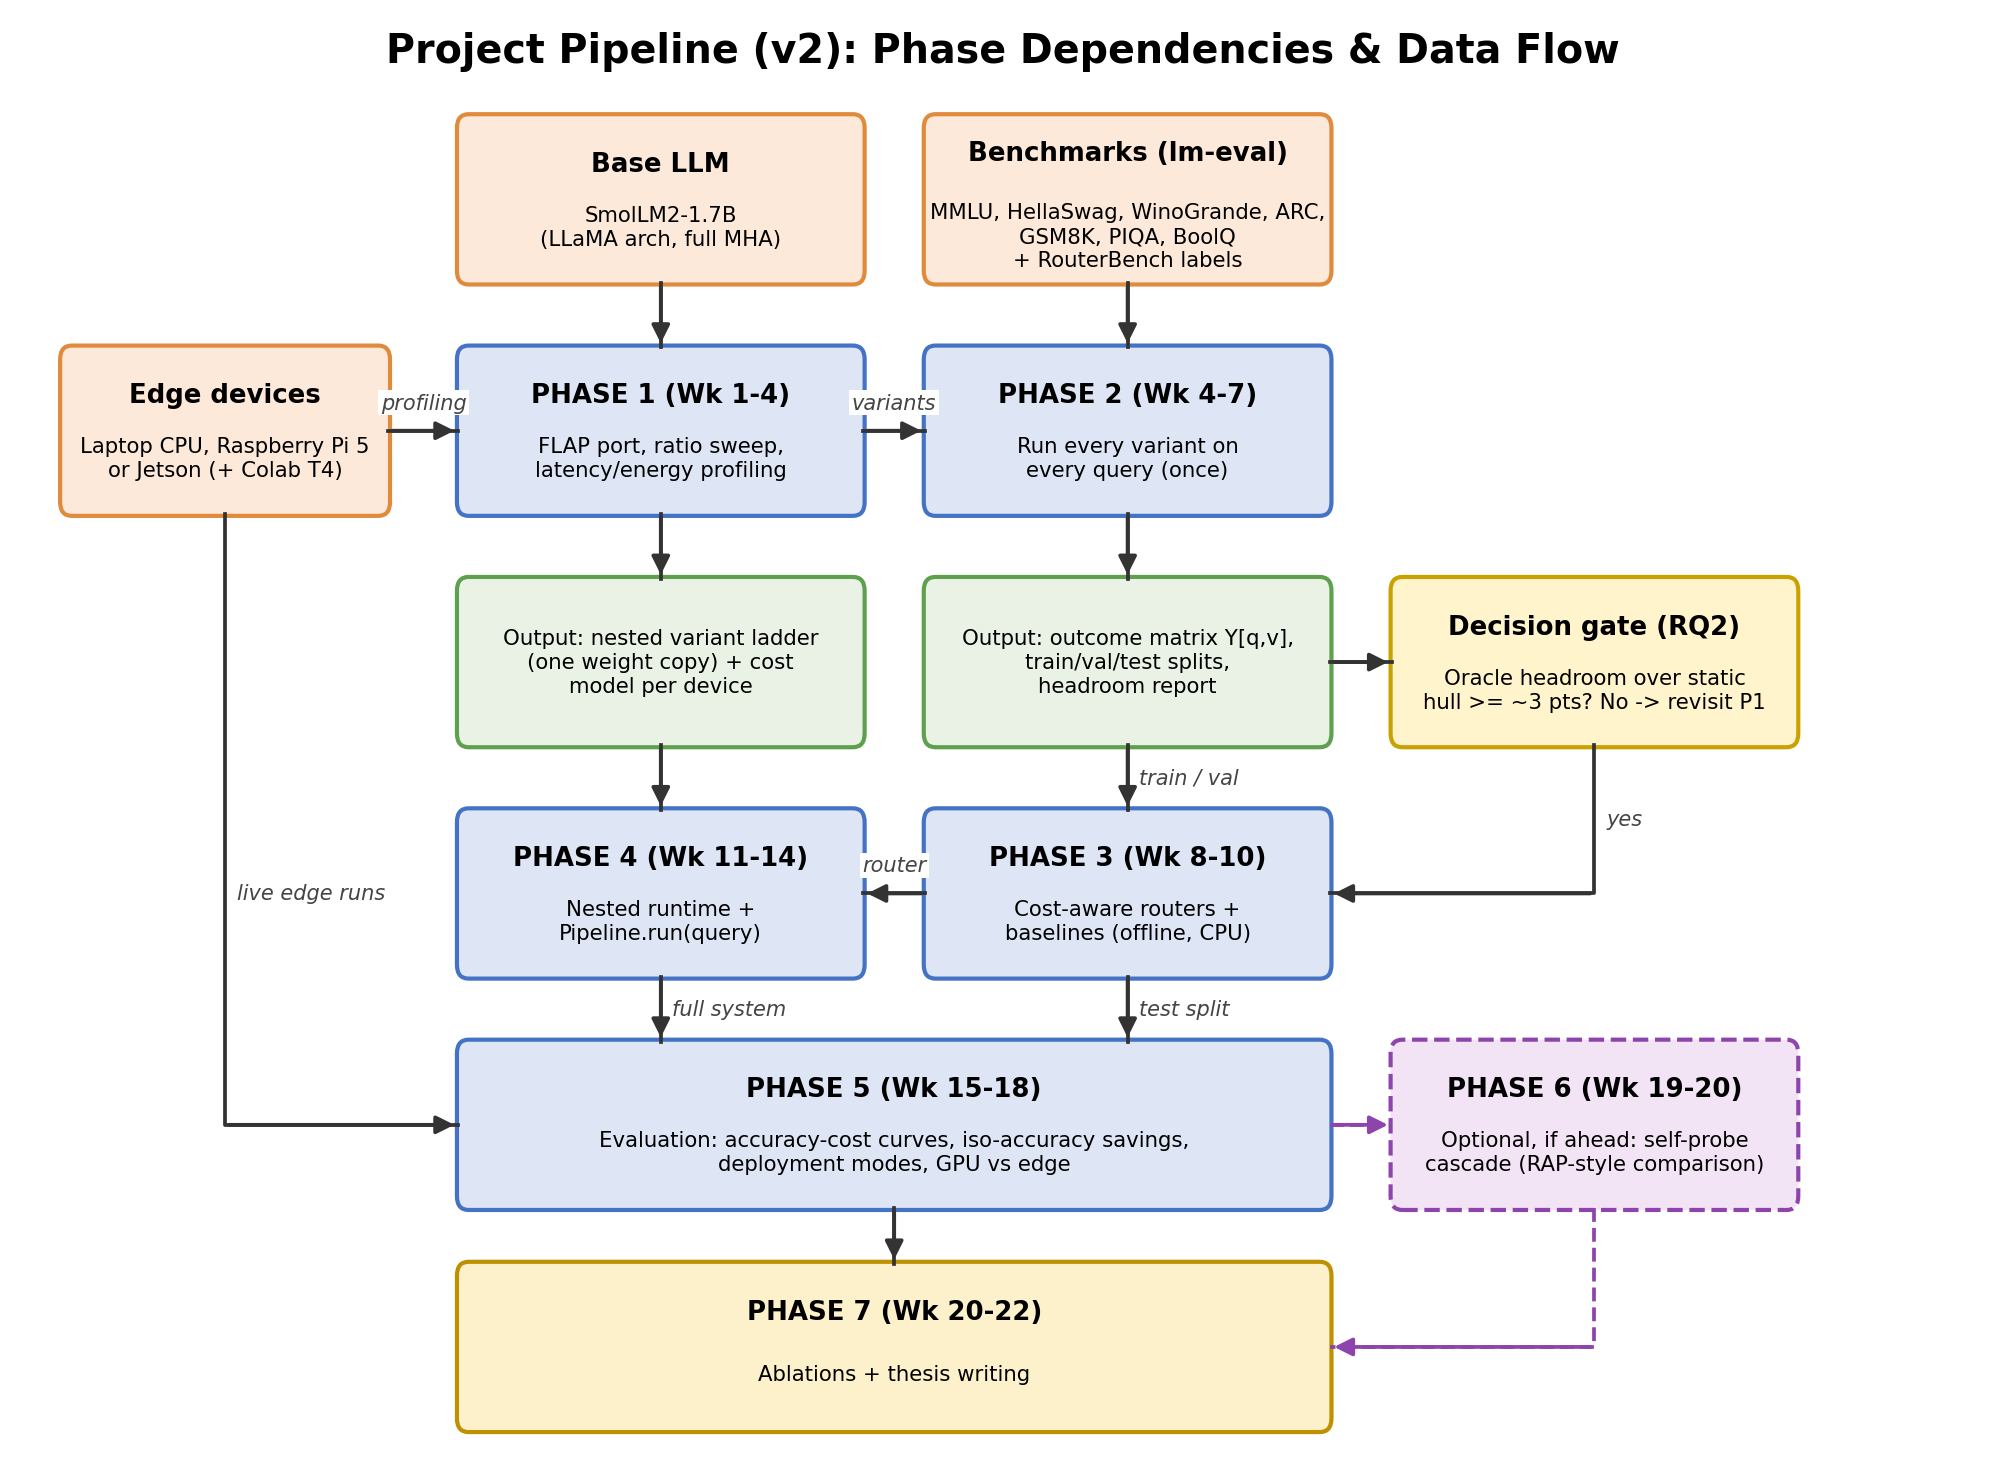
\includegraphics[width=0.92\linewidth]{figures/pipeline_v2.png}
  \caption{Pipeline and phase dependencies. P0--P2 are covered in this report.}
  \label{fig:pipeline}
\end{figure}
Figure~\ref{fig:pipeline} shows the pipeline.
\begin{enumerate}
  \item \textbf{Variant ladder (P1).} FLAP is computed once on the unpruned model; a pruning ratio $r$
  then only selects a threshold. Each variant is stored as a \emph{plan}: per-layer head and channel keep
  masks plus compensation biases ($\approx$0.6\,MB, \texttt{safetensors}), applied to the base weights at load time.
  \item \textbf{Outcome matrix (P2).} Every variant is evaluated once on every query with
  lm-evaluation-harness~\citep{gao2023lmeval}, recording correctness, the log-likelihood of every answer
  option, prompt length and generated length. Routers are then evaluated offline by replaying this
  matrix, so no GPU time is spent per router or per $\lambda$; live runs on a subset will confirm the replay.
  \item \textbf{Routers (P3).} Rule-based, $k$NN, logistic-regression and MLP estimators of $\hat p_v(q)$ on
  MiniLM embeddings plus length/math features, with the decision rule~\eqref{eq:router}; compared with fixed
  variants, the random-mixture hull, a task-type router, a router trained on RouterBench's 11-LLM
  correctness, and the oracle.
  \item \textbf{Runtime (P4) and evaluation (P5).} A shared-weight runtime serves all variants from one
  weight copy; deployment modes (shared / all resident / swap on demand) are compared under a memory budget.
\end{enumerate}

\paragraph{Engineering for correctness.} Every script is seeded and config-driven and writes its
configuration, git commit (with a dirty flag), library versions and logs next to its results. The code
base has 55 automated tests. Problems found and fixed during the work, each now covered by a test, are
listed in Appendix~\ref{app:issues}.

%=======================================================================================
\section{Mathematical Basis}
\label{sec:math}
\subsection{FLAP importance, structure and compensation}
For an output projection $W\in\mathbb R^{d\times m}$ (attention $o$-projection or MLP down-projection)
with input channels $j=1..m$, FLAP accumulates over calibration samples $t=0..N-1$ (each a window of
$T$ tokens, $x_{t,\cdot,j}$) a running mean $\bar x_j$ and a fluctuation $F_j$:
\begin{align}
  \bar x^{(t)}_j &= \tfrac{t}{t+1}\bar x^{(t-1)}_j+\tfrac{1}{t+1}\,\tfrac1T\textstyle\sum_{\tau}x_{t,\tau,j},\\
  F^{(t)}_j &= \tfrac{t-1}{t}F^{(t-1)}_j+\tfrac1{t+1}\textstyle\sum_\tau\big(x_{t,\tau,j}-\bar x^{(t)}_j\big)^2,\qquad F^{(0)}_j=0 .
\end{align}
(The second line is what the official implementation computes: its ``previous mean'' is an alias of the
updated mean, so both factors use $\bar x^{(t)}$; our port reproduces this and a unit test pins it.)
The WIFV score is $S_j=F_j\,\lVert W_{:,j}\rVert_2^2$; attention scores are squared. Scores are standardised
within each layer, $\hat S_j=(S_j-\mu_\ell)/\sigma_\ell$; a head's score is the mean of $\hat S$ over its
$d_h$ channels. All heads and MLP channels of all layers are ranked together and the kept set is
$\{u:\hat S_u>\tau(r)\}$, where $\tau(r)$ is chosen so that the kept parameter weight is closest to $(1-r)$ of
the total, with weight $w_{\text{head}}=\lfloor 4d_h/3\rfloor$ per head and $1$ per MLP channel (a head owns
$4d\,d_h$ parameters, a channel $3d$).

Removing input channels $P$ of a linear layer changes its output $y=W_Kx_K+W_Px_P$; FLAP replaces the
removed term by its calibration expectation, i.e.\ adds the bias
\begin{equation}
  b=W_{:,P}\,\bar x_P .
\end{equation}

\begin{proposition}[Nested variants]\label{prop:nested}
With scores computed once on the unpruned model, the kept sets satisfy $K(r_2)\subseteq K(r_1)$ for
$r_2\ge r_1$.
\end{proposition}
\begin{proof}
The ranking does not depend on $r$. The cumulative kept weight is increasing along the ranking and the
target $(1-r)\sum w$ decreases in $r$, so the selected rank index is non-increasing in $r$ and the
threshold $\tau(r)$ (the score at that index, in descending order) is non-decreasing; a unit with
$\hat S_u>\tau(r_2)$ also has $\hat S_u>\tau(r_1)$.
\end{proof}
Consequently variant $v_r$ is a sub-network of every less-pruned variant, and all variants can be served
from one weight copy plus small per-variant bias vectors. The test suite checks nesting numerically.

\paragraph{Parameter count.} With $h_\ell$ kept heads and $m_\ell$ kept MLP channels in layer $\ell$,
the prunable parameters are $\sum_\ell\big(4\,d\,d_h\,h_\ell+3\,d\,m_\ell\big)$; embeddings are not pruned.

\subsection{Cost and energy}
Batch-1 latency of a query with $n$ prompt tokens and $g$ generated tokens on variant $v$ is modelled as
\begin{equation}
  c(q,v)=\mathrm{prefill}_v(n)+g\cdot\mathrm{decode}_v ,
\end{equation}
with $\mathrm{prefill}_v$ interpolated linearly between measured prompt lengths. Multiple-choice tasks are
scored by log-likelihood, so $g=0$ for them. Energy is $E=\int P\,dt$, read as the difference of the NVML
cumulative energy counter; a 20\,ms power sampler integrated by the trapezoid rule serves as a cross-check.

\subsection{Metrics}
Accuracy uses each task's primary metric (Sec.~\ref{sec:data}). For multiple-choice tasks with option
log-likelihoods $\ell_i$ and character lengths $|o_i|$: $\mathrm{acc}=[\arg\max_i\ell_i=g]$,
$\mathrm{acc\_norm}=[\arg\max_i\ell_i/|o_i|=g]$. Perplexity on WikiText-2 follows FLAP:
non-overlapping 128-token windows, $\mathrm{PPL}=\exp\big(\frac{1}{NT}\sum_w T\cdot\overline{\mathrm{NLL}}_w\big)$.

%=======================================================================================
\section{Experimental Setup}
\label{sec:setup}
\begin{table}[!htbp]
\centering\small
\begin{tabularx}{\linewidth}{lX}
\toprule
Base model & SmolLM2-1.7B (\texttt{HuggingFaceTB/SmolLM2-1.7B}, revision \texttt{effd688a}): Llama architecture, 24 layers,
hidden 2048, 32 attention heads with 32 key/value heads (full multi-head attention), head dim 64, MLP 8192,
no biases, tied embeddings, vocabulary 49{,}152; 1{,}711{,}376{,}384 parameters. \\
GPU & Google Colab, NVIDIA Tesla T4 (16\,GB), fp16, Python 3.13. \\
Edge device & Laptop CPU: Intel Core i5-12500H, 15.6\,GB RAM, Windows 11, PyTorch 2.7.0 (CPU), 12 threads, fp32. \\
Software & transformers 5.17.0, lm-eval 0.4.13, datasets 5.0.1, accelerate 1.15.0, huggingface-hub 1.33.0
(pinned; PyTorch is Colab's build, recorded per run). \\
FLAP settings & As in the official code: WIFV metric, AL-AM structure, WikiText-2~\citep{merity2016wikitext} train
calibration, 1024 windows of 128 tokens, seed 0; PPL with 128-token windows. Ratios 0.1--0.6. \\
Baselines & Wanda-SP and Magnitude-SP at ratios 0.2, 0.35, 0.5 (uniform per layer; Wanda-SP calibrated on
128 WikiText-2 windows instead of C4, so all methods see the same text). \\
Latency protocol & Batch 1, random-token prompts of 128/512/1024 tokens (GPU) or 128/512 (CPU); 64 (GPU) or 32 (CPU)
generated tokens with EOS suppressed; median over 10 (GPU) or 5 (CPU) repetitions after warm-up; CUDA-synchronised; CPU runs require mains power. \\
Seeds & Pool/splits 2026; FLAP calibration 0; lm-eval few-shot seed 2026 for every variant. \\
\bottomrule
\end{tabularx}
\caption{Experimental setup.}
\end{table}

%=======================================================================================
\section{Datasets}
\label{sec:data}
\begin{table}[!htbp]\centering\small
\begin{tabular}{lrrrcccl}
\toprule
Task & Eval docs & Dupes & Kept & Train / Val / Test & Metric & Shots & HF dataset \\
\midrule
ARC-Easy & 2{,}376 & 0 & 2{,}376 & 1{,}426 / 475 / 475 & acc & 0 & \texttt{allenai/ai2\_arc} \\
ARC-Challenge & 1{,}172 & 0 & 1{,}172 & 703 / 234 / 235 & acc\_norm & 0 & \texttt{allenai/ai2\_arc} \\
HellaSwag & 10{,}042 & 0 & 4{,}000 (cap 4{,}000) & 2{,}400 / 800 / 800 & acc\_norm & 0 & \texttt{Rowan/hellaswag} \\
WinoGrande & 1{,}267 & 0 & 1{,}267 & 760 / 253 / 254 & acc & 0 & \texttt{allenai/winogrande} \\
PIQA & 1{,}838 & 0 & 1{,}838 & 1{,}103 / 368 / 367 & acc & 0 & \texttt{baber/piqa} \\
BoolQ & 3{,}270 & 0 & 3{,}270 & 1{,}962 / 654 / 654 & acc & 0 & \texttt{aps/super\_glue} \\
MMLU & 14{,}042 & 105 & 4{,}000 (cap 4{,}000) & 2{,}397 / 803 / 800 & acc & 0 & \texttt{cais/mmlu} \\
GSM8K & 1{,}319 & 0 & 1{,}319 & 791 / 264 / 264 & exact match & 5 & \texttt{openai/gsm8k} \\
\midrule Total & & & 19{,}242 & 11{,}542 / 3{,}851 / 3{,}849 & & & \\
\bottomrule
\end{tabular}
\caption{Query pool (lm-eval 0.4.13, seed 2026). Dataset revisions (Hub commit hashes) are recorded in \texttt{data/p2/manifest.json}.}
\label{tab:pool}
\end{table}


The query pool is built from lm-eval's own task definitions, so document order, gold labels and prompts
are exactly those that lm-eval evaluates; each row stores lm-eval's document hash and the outcome
parser rejects any logged sample whose hash differs. Exact duplicates (same question and options) are
dropped (105 in MMLU). MMLU~\citep{hendrycks2021mmlu} is capped at 4{,}000 questions allocated to subjects
in proportion to their size, HellaSwag~\citep{zellers2019hellaswag} at 4{,}000 uniformly; the other tasks
(ARC-Easy/Challenge~\citep{clark2018arc}, WinoGrande~\citep{sakaguchi2019winogrande}, PIQA~\citep{bisk2020piqa},
BoolQ~\citep{clark2019boolq}, GSM8K~\citep{cobbe2021gsm8k}) are used in full. Each task (and each MMLU subject)
is split 60/20/20 into train/validation/test with seed 2026; rebuilding the pool reproduces it exactly.

\paragraph{Scoring.} Multiple-choice tasks are zero-shot and scored by option log-likelihood, with
acc\_norm as the primary metric for HellaSwag and ARC-Challenge and acc elsewhere (the LLM-Pruner/FLAP
reporting convention); both are stored. GSM8K is 5-shot with greedy generation capped at 256 tokens;
an answer is correct if the extracted number matches (lm-eval's \emph{flexible-extract} filter); strict
match is stored too.

\paragraph{External difficulty labels (RouterBench).}
RouterBench~\citep{hu2024routerbench} (0-shot file, revision \texttt{78402148}, SHA-256 \texttt{ba4f77f19517}\ldots) records whether each of 11 LLMs answered a prompt correctly. We attach the mean correctness over these models to our queries as an \emph{external} difficulty label, used only in a later ablation. The file is a Python pickle; it is loaded with a restricted unpickler that permits only 11 pandas/numpy reconstruction functions. Questions are matched by content with answer options sorted, because RouterBench shuffles option order. Queries whose key occurs in RouterBench with different scores are left unlabelled. In total 10{,}420 of our queries are labelled (Table~\ref{tab:rb}).

\begin{table}[!htbp]\centering\small
\begin{tabular}{lrrrrl}
\toprule
Task & Pool & RouterBench rows & Matched & Ambiguous & Note \\
\midrule
HellaSwag & 4{,}000 & 10{,}042 & 4{,}000 & 0 &  \\
WinoGrande & 1{,}267 & 1{,}267 & 1{,}267 & 0 &  \\
ARC-Challenge & 1{,}172 & 1{,}470 & 1{,}172 & 0 &  \\
MMLU & 4{,}000 & 14{,}042 & 3{,}981 & 19 &  \\
GSM8K & 1{,}319 & 7{,}450 & 0 & 0 & RouterBench uses the GSM8K train split \\
ARC-Easy & 2{,}376 & 0 & 0 & -- & task not in RouterBench \\
PIQA & 1{,}838 & 0 & 0 & -- & task not in RouterBench \\
BoolQ & 3{,}270 & 0 & 0 & -- & task not in RouterBench \\
\bottomrule
\end{tabular}
\caption{Matching our pool to RouterBench.}\label{tab:rb}
\end{table}


%=======================================================================================
\section{Results and Analysis}
\label{sec:results}
\subsection{Measurement infrastructure (P0)}
On the Colab Tesla T4 all environment checks passed: seeding reproduced identical tensors; a model whose layers have different numbers of heads and MLP channels plus compensation biases (the shape FLAP produces) gave the same logits whether pruned physically or by masking, in fp32 and fp16 and with eager and SDPA attention (maximum fp16 logit difference 0.0). The NVML energy counter is supported on the T4 and agrees with the independent 20\,ms power sampler to within 1.7\% at idle (30.2\,J vs.\ 30.7\,J over 3.0\,s, mean 10.2\,W) and 1.1\% under an fp16 matrix-multiply load (692.4\,J vs.\ 700.0\,J over 10.0\,s, mean 69.7\,W, 23.6\,TFLOPS). Energy figures in this work therefore use the counter.

\subsection{Pruned-variant ladder (P1)}
\pend{the FLAP sweep (ratios 0.1--0.6) and the Wanda-SP / Magnitude-SP baselines are running on the Colab T4; perplexity, parameter counts and GPU latency will be reported from \texttt{results/p1/<run>/sweep.csv}.}

\paragraph{Edge device (laptop CPU).} Table~\ref{tab:cpu} gives batch-1 latency on the Intel i5-12500H in fp32 (median of 3 repetitions after one warm-up). CPU energy is not measured yet (no power measurement is implemented for this laptop).

\begin{table}[h]\centering\small
\begin{tabular}{lrrrrr}
\toprule
Variant & Params (B) & Weights (GB, fp32) & Prefill 128 (s) & Prefill 512 (s) & Decode (ms/tok) \\
\midrule
unpruned & 1.711 & 6.38 & 2.84 & 9.02 & 498 \\
\bottomrule
\end{tabular}
\caption{Laptop-CPU latency (fp32, batch 1, 12 threads).}\label{tab:cpu}
\end{table}
\pend{CPU profiles of the pruned variants, which need the plans produced by the T4 sweep.}

\subsection{Accuracy and oracle headroom (P2)}
\pend{per-variant accuracy on all 19{,}242 queries and the headroom analysis of Eq.~\eqref{eq:headroom}; the outcome runs for the unpruned model and the FLAP variants are queued on the T4 after the sweep.}



%=======================================================================================
\section{Conclusion and Plan}
\label{sec:plan}
\paragraph{What worked.}
\begin{itemize}
\item \emph{FLAP reproduces on a small edge model.} On SmolLM2-1.7B the ranking FLAP $<$ Wanda-SP $<$ Magnitude-SP in perplexity holds at every ratio tested, as the FLAP paper reports for LLaMA models of 7\,B parameters and larger. Light pruning is cheap in quality: FLAP-10\% moves WikiText-2 perplexity only from 18.48 to 20.82.
\item \emph{Pruning gives measurable resource savings on the GPU.} At 50\%, energy per generated token falls by 27\% (2.09 to 1.52\,J), peak memory from 6.48 to 5.00\,GB, and prefill latency by 35\% (512 tokens) and 38\% (1024 tokens).
\item \emph{Per-query routing has real, if small, headroom.} After excluding every variant that does not beat a constant answer, the oracle still exceeds the best fixed variant by 1.9 points (64.1\% to 66.1\%) at the same cost, with gains on PIQA $+$5.2, ARC-Easy $+$4.6, GSM8K $+$4.2, HellaSwag $+$2.8. On PIQA, FLAP-50\% keeps 60.8\% accuracy (constant answer: 50.1\%) with 47\% fewer parameters.
\item \emph{A method that prevents an overclaim.} The plain oracle would suggest a routing gain of 11.7 points; most of it comes from variants that answer every question identically. The informative oracle introduced here measures the gain a router could actually exploit.
\item \emph{Reliable infrastructure.} Results are identical question by question across runs on different days; every result is cross-checked against lm-eval; several silent errors that would have corrupted results were found and fixed (Appendix~\ref{app:issues}).
\end{itemize}
\paragraph{What did not work.}
\begin{itemize}
\item Accuracy falls steeply: macro accuracy 62.5\% (unpruned) to 47.3\% (20\%), 40.0\% (35\%) and 32.6\% (50\%). The most frequent MMLU answer covers 100\% of questions for FLAP-35\% and 100\% for FLAP-50\% (unpruned: 32\%), and on GSM8K the pruned variants reach the 256-token limit on 80--100\% of questions.
\item On the T4 at batch size 1, decode latency stays at 30.4--31.1\,ms per token for every ratio, so pruning does not shorten generation there; with similar multiple-choice costs and longer GSM8K outputs, per-query routing saves no latency on this GPU.
\item Laptop-CPU timings were not reliable enough to report (Section~\ref{sec:results}).
\end{itemize}
\paragraph{What is next.} The results point to concrete steps: evaluating milder ratios (10--30\%) to test whether the pruned variants stay above the constant-answer baseline on more tasks; removing the per-token overhead on the GPU (static KV cache with CUDA graphs) and int8 weights on the CPU, both implemented and unit-tested but not yet measured; and a controlled CPU measurement. The remaining phases are planned as follows.


\begin{table}[!htbp]
\centering\small
\begin{tabular}{p{2.6cm}p{2.3cm}p{9.6cm}}
\toprule
Dates (2026) & Work package & Tasks and deliverable \\
\midrule
22 Oct -- 28 Oct & Better cheap variants &
\emph{Done in part:} in-domain-calibrated FLAP at 10/20/35\% and FLAP 10\% evaluated on the test split
(Table~\ref{tab:calib}). Remaining: in-domain calibration at 30\% and 50\%; choose the ladder for the rest of the thesis.
\emph{Deliverable:} variant set for the rest of the thesis. \\
29 Oct -- 4 Nov & Cascade fix &
Token-level cascade (speculative decoding): pruned, int8 draft of the model, unpruned model verifies; greedy output
must be identical to the unpruned model. Sweep draft ratio (10--50\%), draft length (3--8 tokens) and the draft's
confidence stop; paired, drift-robust timing on the laptop CPU and on the T4.
\emph{Deliverable:} speed-up with 95\% CI at identical output. \\
5 Nov -- 11 Nov & Faster execution &
Static KV cache + CUDA graphs on the T4; int8 weights and P-core thread pinning on the CPU; controlled CPU latency
measurement in an idle window. Optional short LoRA recovery of the pruned variants if accuracy is still too low.
\emph{Deliverable:} measured cost model per device. \\
12 Nov -- 18 Nov & Routers &
Outcome runs on train/validation; rule-based, $k$NN, logistic-regression and MLP routers on query-text features;
task-type and RouterBench-trained baselines; offline replay against the informative oracle.
\emph{Deliverable:} accuracy--cost curves on the test split. \\
19 Nov -- 25 Nov & Pipeline and evaluation &
Shared-weight runtime and \texttt{Pipeline.run} combining the router with the token-level cascade; live validation of
the offline replay and cost model on the T4 and the laptop CPU; iso-accuracy savings, memory-budget scenario,
bootstrap CIs. \emph{Deliverable:} final results tables and figures. \\
26 Nov -- 2 Dec & Ablations and writing &
Calibration source, ratio set, draft length, int8 on/off; write all thesis chapters from the generated tables. \\
3 Dec -- 5 Dec & Buffer and submission &
Proof-reading, final regeneration of every table and figure from \texttt{results/}, submission on 5 December. \\
\bottomrule
\end{tabular}
\caption{Remaining work until the final submission (5 December 2026).}
\end{table}

\appendix
\section{Problems found and fixed}
\label{app:issues}
\begin{enumerate}
  \item lm-eval 0.4.13 maps results selected with \texttt{samples=} back by position, which is correct only
  for sorted indices; unsorted indices would silently attach results to the wrong questions. Indices are
  now sorted and every sample's document hash is checked.
  \item RouterBench shuffles answer options relative to the source datasets; order-sensitive matching
  matched only $\approx$4\% of MMLU/HellaSwag/ARC questions and exactly 50\% of WinoGrande. Matching is now
  order-invariant.
  \item RouterBench stores GSM8K prompts as a list of exemplars followed by the question, which caused all
  7{,}450 GSM8K prompts to fail parsing; after the fix, it was verified that RouterBench's GSM8K items are
  the GSM8K \emph{train} split (7{,}450 of 7{,}473 found; 0 of 1{,}319 test questions).
  \item Runs made inside the repository were recorded as having uncommitted changes because the run's own
  output folder was counted; the git state is now read before the run folder is created.
  \item The official FLAP code hard-codes head dimension 128 and the head weight $512/3$ (LLaMA-7B values) and
  writes to bias tensors that bias-free models do not have; the port generalises all three.
  \item CPU timings taken on battery power were throttled and inconsistent; they were discarded and profiling now
  refuses to run on battery.
  \item Pruned variants that always give the same answer made the plain oracle reach 100\% on BoolQ; the analysis
  now also reports an informative oracle that only admits variants beating a constant answer.
  \item A Python environment under the Windows Temp folder was partly deleted by temp cleanup in the middle of a run;
  the environment now lives inside the project folder.
\end{enumerate}

\bibliographystyle{plainnat}
\bibliography{refs}
\end{document}
